\documentclass[12pt, a4papre]{article}
\usepackage[catalan]{babel}
\usepackage[unicode]{hyperref}
\usepackage{amsmath}
\usepackage{amssymb}
\usepackage{amsthm}
\usepackage{xifthen}
\usepackage{listings}
\usepackage{float}
\usepackage{siunitx}
\usepackage{graphicx}
\usepackage{indentfirst}

\newcommand{\norm}[1]{\lvert #1 \rvert}
\graphicspath{ {./Images/} }

\hypersetup{
    colorlinks = true,
    linkcolor = blue
}

\author{Daniel Vilardell}
\title{Previ practica 2}
\date{}

\begin{document}
	\maketitle
	
	\textbf{Qüestió 1: }Savem que la formula per a calcular la impedancia de un condensador es $Z = \frac{1}{jCw}$ per tant en el nostre cas serà:
	
	\[
		|Z_1| = |\frac{1}{jC_1w}| =  |\frac{1}{jC_12\pi f}| = \frac{1}{10\cdot 10^{-9}\cdot 2\pi \cdot40 \cdot 10^{3}} =  \SI{397.9}{\ohm}
	\]
	\[
		|Z_2| = |\frac{1}{jC_2w}| =  |\frac{1}{jC_22\pi f}| = \frac{1}{10\cdot 10^{-6}\cdot 2\pi \cdot40 \cdot 10^{3}} =  \SI{0.4}{\ohm}
	\]
	
	\textbf{Qüestió 2: }
	\begin{figure}[H]
		\begin{center}
		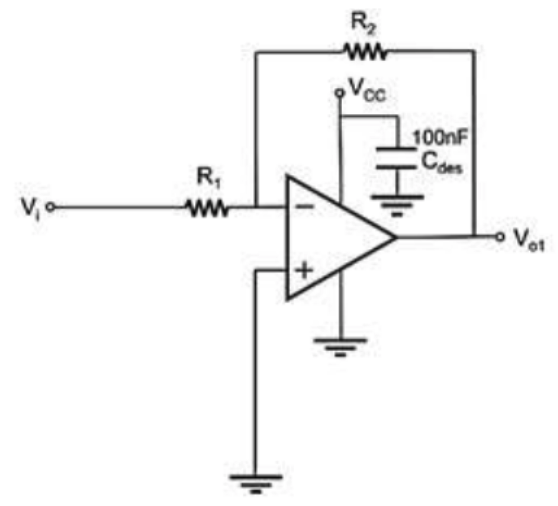
\includegraphics[width=60mm]{previ2_2.png}
		\caption{Circuit amb una entrada de 40kHz}
		\end{center}
	\end{figure}
	
	\textbf{Qüestió 3: }El circuit es un inversor com els que ja hem vist molts cops i per tant el guany serà
	
	\[
		G = \frac{R_2}{R_1}
	\]
	
	\textbf{Qüestió 4: }La freqüencia de guany unitat es el producte entre el guany i l'ample de banda, i per tant
	
	\[
		f_t = G \cdot BW = 400 \cdot 40 \cdot 10^3 = 16MHz
	\]
	
	\textbf{Qüestió 5: } 
	\begin{figure}[H]
		\begin{center}
		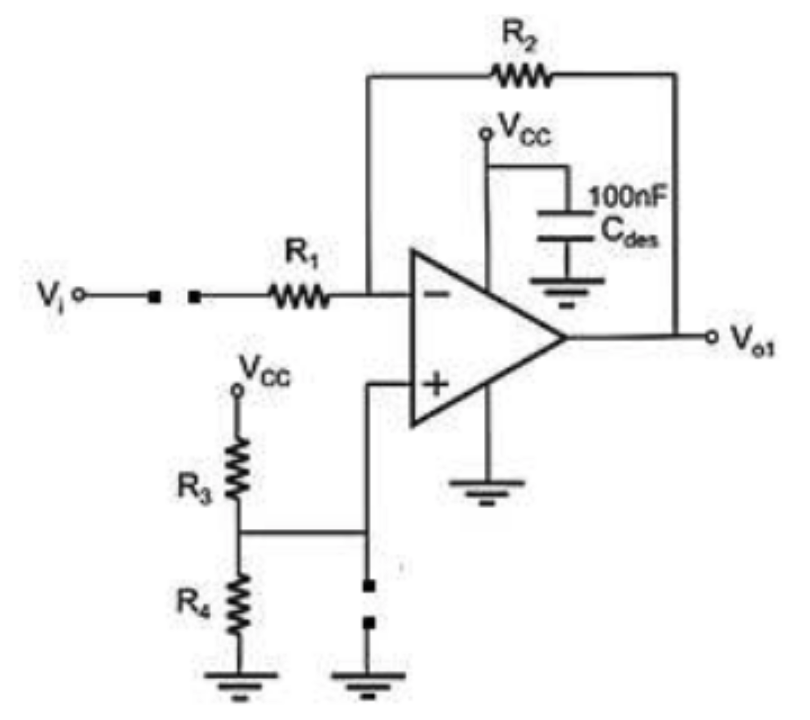
\includegraphics[width=60mm]{previ2_5.png}
		\caption{Circuit amb una entrada continua}
		\end{center}
	\end{figure}
	
	El circuit per tant passa a ser un divisor de tensió i la sortida es
	\[
		V_0 = \frac{R_4}{R_3 + R_4}V_{cc}
	\]
	\textbf{Qüestió 6: }En primer lloc podem trobar el valor de la suma $R_3 + R_4$.
	
	\[
		I = \frac{V_{cc}}{R_3 + R_4} \implies R_3 + R_4 = \frac{V_{cc}}{I} = \SI{120}{k\ohm}
	\]
	
	Com hem vist al apartat anterior també sabem que 
	\[
		V_0 = \frac{R_4}{R_3 + R_4}V_{cc} \implies \frac{V_0}{V_{cc}} = \frac{R_4}{R_3 + R_4} = \frac{1}{2}
	\]
	I d'aquí veiem que $R_3 = R_4 = \SI{60}{k\ohm}$.
	
	\textbf{Qüestió 7: } 
	
	\[
		SR = wV_{0 max} = 2\pi fV_{0 max} = 2\pi\cdot 40 \cdot 10^3 \cdot 12 = 3.02 \frac{V}{\mu s}
	\]
	\newpage
	\textbf{Qüestió 8: } 
	\begin{itemize}
		\item El número d'AO que conté el xip: 2
		\item El tipus d'alimentació que admet: 15 a 12 V
		\item La freqüencia de guany unitat $f_t$: 4.5 MHz
		\item El slew-rate SR de l'AO: 9$ \frac{V}{\mu s}$
	\end{itemize}
	
	\textbf{Qüestió 9: }El AO que ens proporciona el laboratori te una $f_t$ de 4.5 MHz pero hem vist al apartat 4 que necessitem 16MHz, per tant si en coloquem 2 en cascada aconseguirem obtenir $4.5^2 = 20.25 MHz > 16 MHz$.
	
	\textbf{Qüestió 10: }Per tal que la impedancia de $C_1$ no afecti escollirem una $R_1$ 100 vegades mes gran que aquesta, per tant $R_1 = \SI{40}{k\ohm}$. Com que $G_1G_2 = 400$ on $G_1$ i $G_2$ son els guanys en les 2 fases tenim que si considerem  
	\[
		G_1 = G_2 = 20 \implies \frac{R_2}{R_1} = 20 \implies R_2 = \SI{800}{k\ohm}
	\]
	
	\textbf{Qüestió 11: }El dibuix del circuit serà agafar 2 cops el circuit donat al enunciat i posarlo en cascada de la següent forma
	\begin{figure}[H]
		\begin{center}
		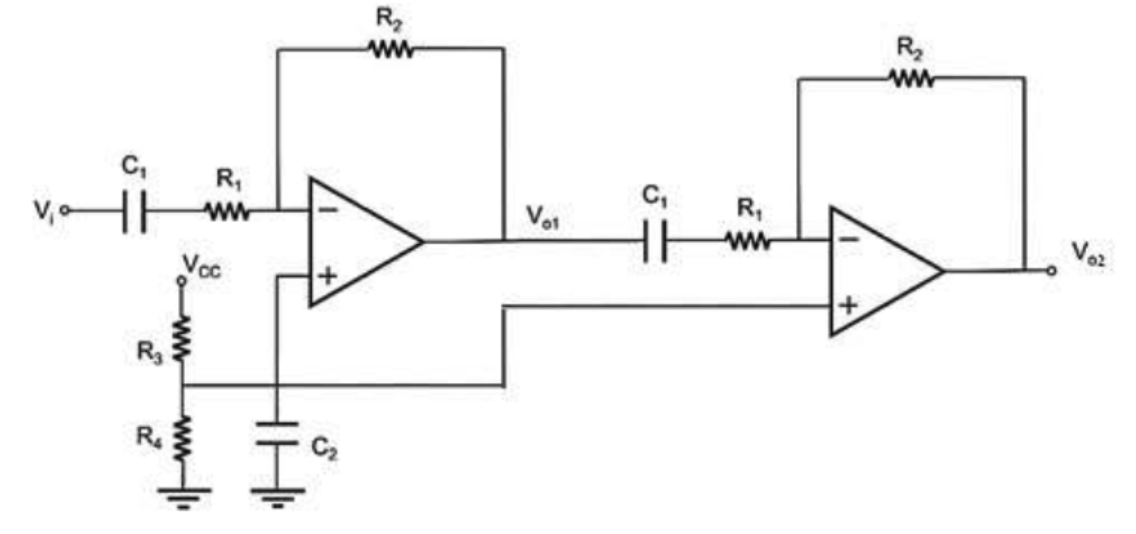
\includegraphics[width=100mm]{previ2_11.png}
		\caption{Circuit final}
		\end{center}
	\end{figure}
	
\end{document}




